\documentclass[border=10pt]{standalone}

\usepackage{tikz}
\usepackage{tikzsymbols}
\usetikzlibrary{calc,patterns,shapes.geometric}

\def\centerarc[#1](#2)(#3:#4:#5){\draw[#1] ($(#2)+({#5*cos(#3)},{#5*sin(#3)})$) arc (#3:#4:#5);}

\begin{document}
	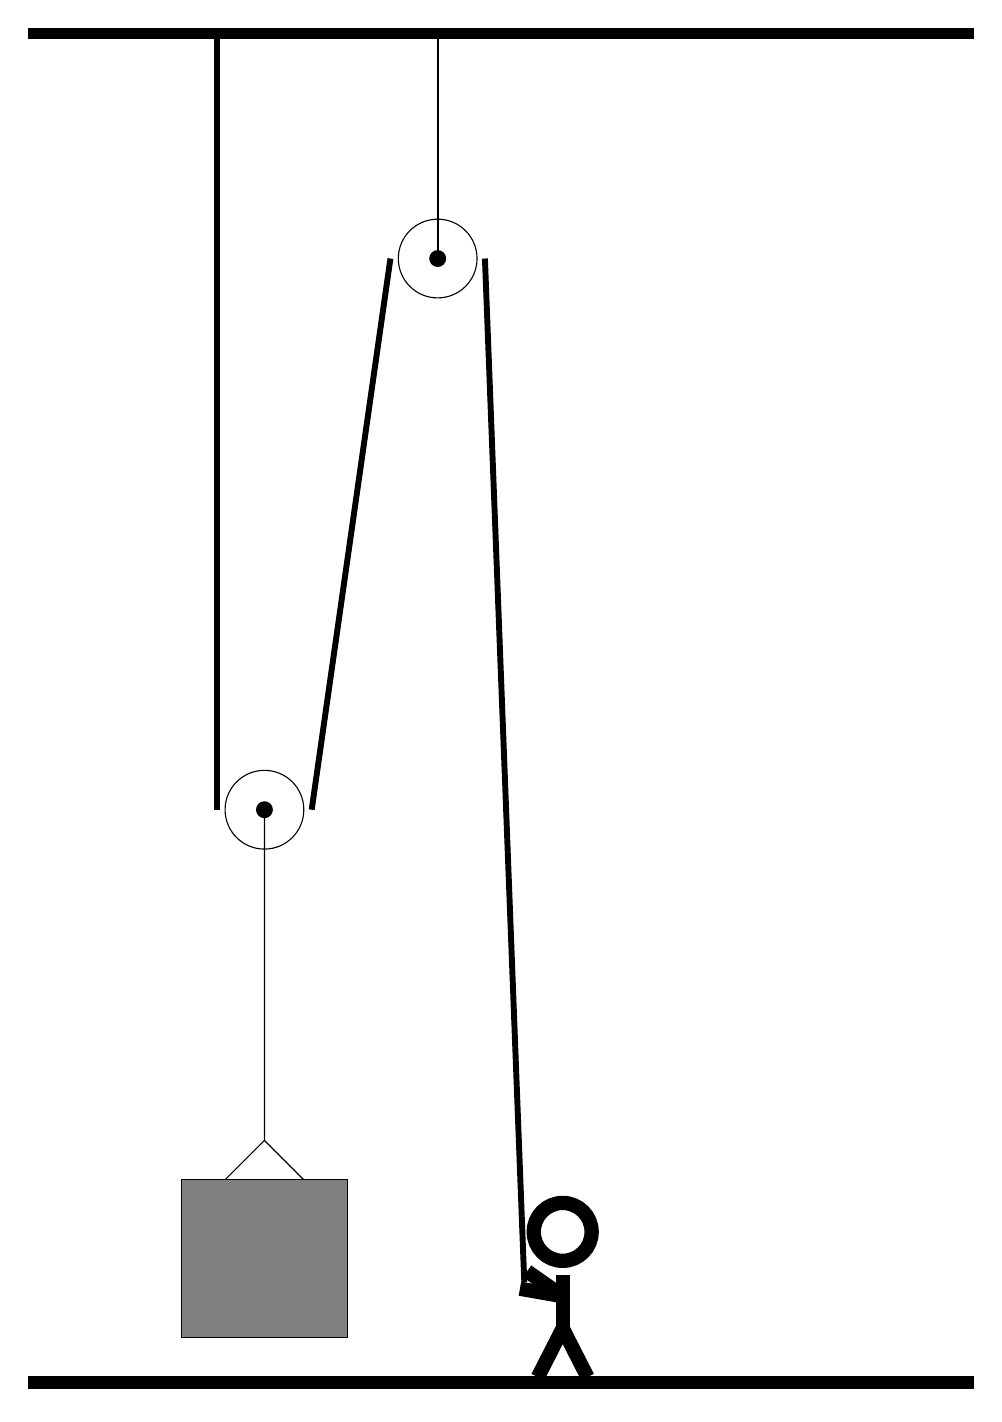
\begin{tikzpicture}
		%%%%% START %%%%%
		\draw[fill=black] (-2, 14) rectangle (10, 14.125);
		
		\draw (3.2, 11.2) circle (0.5);
		\draw[fill=black] (3.2, 11.2) circle (0.1);
		\draw[thick] (3.2, 11.2) -- (3.2, 14);
		
		\draw (1, 4.2) circle (0.5);
		\draw[fill=black] (1, 4.2) circle (0.1);
		
		\draw (1, 4.2) -- (1, 0) -- (0.5, -0.5);
		\draw (1, 0) -- (1.5, -0.5);
		\draw[fill=black!50] (-0.05, -0.5) rectangle (2.05, -2.5);
		
		\draw[line width=0.75mm] (0.4, 14) -- (0.4, 4.2);
		\centerarc[line width=0.75mm](1, 4.2)(180:360:0.6);
		\draw[line width=0.75mm](1.6, 4.2) -- (2.6, 11.2);
		\centerarc[line width=0.75mm](3.2, 11.2)(0:180:0.6);
		\draw[line width=0.75mm](3.8, 11.2) -- (4.3, -1.8);
		
		\node at (4.7, -1.9) {\Strichmaxerl[10][-35][170]};
		
		\draw[fill=black] (-2, -3) rectangle (10, -3.15);
		%%%%% END %%%%%
	\end{tikzpicture}
\end{document}